\documentclass[a4paper,10pt,foldmark,notumble]{leaflet}

% Compile with XeLaTeX!!!
\usepackage{ifxetex}
\ifxetex
\pdfpagewidth=3\paperwidth
\pdfpageheight=\paperheight
\usepackage{fontspec}
\defaultfontfeatures{Mapping=tex-text}
\input{UBScala/fontspec}
\setmainfont{UBScala}
\setsansfont{UBScalaSans}
\else
\fi

\usepackage[dvipsnames,usenames]{xcolor}
%%UNIBA-Colors
\definecolor{unibablueI}{HTML}{00457D}
\definecolor{unibablueII}{HTML}{336A97}
\definecolor{unibablueIII}{HTML}{6690B1}
\definecolor{unibablueIV}{HTML}{99B5CB}
\definecolor{unibablueV}{HTML}{CCDAE5}

\definecolor{unibayellowI}{HTML}{FFD300}
\definecolor{unibayellowII}{HTML}{FFDC33}
\definecolor{unibayellowIII}{HTML}{FFE566}
\definecolor{unibayellowIV}{HTML}{FFED99}
\definecolor{unibayellowV}{HTML}{FFF6CC}

\definecolor{unibagreenI}{HTML}{97BF0D}
\definecolor{unibagreenII}{HTML}{ACCC3D}
\definecolor{unibagreenIII}{HTML}{C1D86E}
\definecolor{unibagreenIV}{HTML}{D5E59E}
\definecolor{unibagreenV}{HTML}{EAF2CF}
%Not CD, darker versions
\definecolor{nounibagreenI}{HTML}{82A50B}
\definecolor{nounibagreenII}{HTML}{708C0A}

\definecolor{unibaredI}{HTML}{E6444F}
\definecolor{unibaredII}{HTML}{EB6972}
\definecolor{unibaredIII}{HTML}{F08F95}
\definecolor{unibaredIV}{HTML}{F5B4B8}
\definecolor{unibaredV}{HTML}{FADADC}
%Not CD, darker versions
\definecolor{nounibaredI}{HTML}{CC3D47}
\definecolor{nounibaredII}{HTML}{B3363E}

\definecolor{unibagrayI}{HTML}{878783}
\definecolor{unibagrayII}{HTML}{9F9F9C}
\definecolor{unibagrayIII}{HTML}{B7B7B5}
\definecolor{unibagrayIV}{HTML}{CFCFCE}
\definecolor{unibagrayV}{HTML}{E7E7E6}

%%%%%%%%%%%%%%%%%%%%%%%%%%%%%%%%%%%%%%%%%%%%%%%%%%%%%%%%%%%
% TIKZ Configuration
%%%%%%%%%%%%%%%%%%%%%%%%%%%%%%%%%%%%%%%%%%%%%%%%%%%%%%%%%%%
\usepackage{tikz}
\usetikzlibrary{positioning,patterns,calc}


\renewcommand*\foldmarkrule{.3mm}
\renewcommand*\foldmarklength{5mm}

\usepackage{amsmath}
%\usepackage[T1]{fontenc}
\usepackage{textcomp}
\usepackage{mathptmx}
%\usepackage[scaled=0.9]{helvet}
\makeatletter
\def\ptmTeX{T\kern-.1667em\lower.5ex\hbox{E}\kern-.075emX\@}
\DeclareRobustCommand{\ptmLaTeX}{L\kern-.3em
        {\setbox0\hbox{T}%
         %\vb@xt@ % :-)
         \vbox to\ht0{\hbox{%
                            \csname S@\f@size\endcsname
                            \fontsize\sf@size\z@
                            \math@fontsfalse\selectfont
                            A}%
                      \vss}%
        }%
        \kern-.12em
        \ptmTeX}
\makeatother
%\let\TeX=\ptmTeX
%\let\LaTeX=\ptmLaTeX
\usepackage{shortvrb}
%\MakeShortVerb{\|}
\usepackage{url}
\usepackage{graphicx}
\usepackage{longtable}
\usepackage{colortbl}
\usepackage{multirow,varwidth,array}
\definecolor{LIGHTGRAY}{gray}{.9}

%%%%\renewcommand{\descfont}{\normalfont}
\newcommand\Lpack[1]{\textsf{#1}}
\newcommand\Lclass[1]{\textsf{#1}}
\newcommand\Lopt[1]{\texttt{#1}}
\newcommand\Lprog[1]{\textit{#1}}

\newcommand*\defaultmarker{\textsuperscript\textasteriskcentered}

%\usepackage[colorlinks=true, urlcolor=unibablueI]{hyperref}

\title{\bf MMB \& DFT 2014}

\author{%
\Large \bf University of Bamberg
%  Martin Schmoll\\
%  Predrag Puno\v{s}evac
}
\date{\bf March 17 -- 19, 2014 }

\CutLine*{1}
\CutLine*{6}

%\AddToBackground{1}{%  Background of a small page
%  \put(0,0){\textcolor{Cerulean}{\rule{\paperwidth}{\paperheight}}}}


%\AddToBackground{1}{%  Background of a small page
%  \put(115,530){\includegraphics[scale=0.12]{tiger.eps}}}


\AddToBackground{6}{%  Background of a small page
  \put(0,0){\textcolor{unibablueV}{\rule{\paperwidth}{\paperheight}}}}


%\AddToBackground*{2}{% Background of a large page
%  \put(\LenToUnit{.5\paperwidth},\LenToUnit{.5\paperheight}){%
%    \makebox(0,0)[c]{%
%      \resizebox{.9\paperwidth}{!}{\rotatebox{35.26}{%
%        \textsf{\textbf{\textcolor{LIGHTGRAY}{CLEMSON}}}}}}}}


\begin{document}
\maketitle

\newpage
%\section{Time Table}

\newcommand{\daywidth}{24mm}
\newcommand{\daytextwidth}{21mm}

\newcommand{\hourseparation}{3mm}

\begin{tikzpicture}[yscale=-0.1, xscale=0.1, node distance=1mm,outer sep = 0pt]

% Style for Days
\tikzstyle{day}=[draw, white, rectangle,  minimum height=5mm, minimum width=\daywidth, fill=unibablueI,anchor=north west, align=center, font=\small]
% Style for hours
\tikzstyle{hour}=[draw, rectangle, minimum height=5mm, minimum width=8mm, fill=unibagrayIV, anchor=north west, align=center, font=\scriptsize]

\tikzstyle{default}=[anchor=north west,draw=red]

% Styles for events
% Duration of sequences
\tikzstyle{hours}=[rectangle,draw, minimum width=\daywidth, text width=\daytextwidth, anchor=north west, align=center, font=\footnotesize]
\tikzstyle{hhours}=[rectangle,draw, minimum width=.5*\daywidth-1.5mm, text width=.5*\daytextwidth-1.5mm, anchor=north west, align=center, font=\footnotesize]

\tikzset{grid/.style={gray,very thin,opacity=1}}

%\node[default] at (-7,-12) {
%        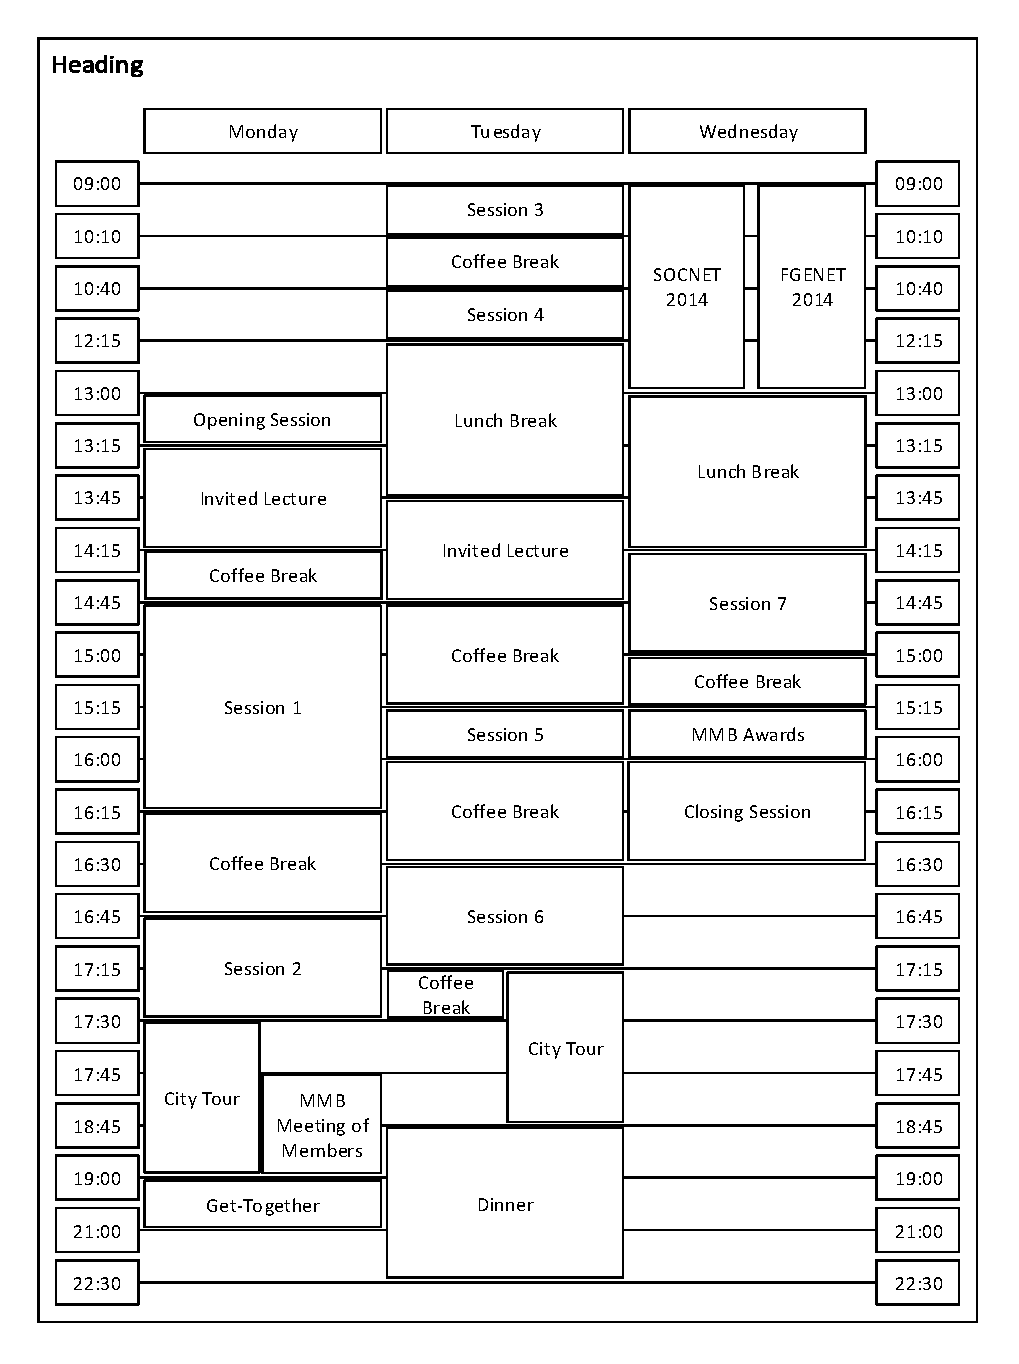
\includegraphics[width=2cm+\textwidth]{images/timetable.pdf}
%    };
    
%\draw[grid] (0,0) grid (10*\textwidth,10*\textheight);

\node[day] (mo) at (9,0) {Monday};
\node[day] (tu) [right = of mo] {Tuesday};
\node[day] (we) [right = of tu] {Wednesday};

\node[hour] (0900) at (0,7) {09:00};
\node[hour] (1010) [below = \hourseparation of 0900] {10:10};
\node[hour] (1040) [below = \hourseparation of 1010] {10:40};
\node[hour] (1215) [below = \hourseparation of 1040] {12:15};
\node[hour] (1300) [below = \hourseparation of 1215] {13:00};
\node[hour] (1315) [below = \hourseparation of 1300] {13:15};
\node[hour] (1345) [below = \hourseparation of 1315] {13:45};
\node[hour] (1415) [below = \hourseparation of 1345] {14:15};
\node[hour] (1445) [below = \hourseparation of 1415] {14:45};
\node[hour] (1500) [below = \hourseparation of 1445] {15:00};
\node[hour] (1515) [below = \hourseparation of 1500] {15:15};
\node[hour] (1600) [below = \hourseparation of 1515] {16:00};
\node[hour] (1615) [below = \hourseparation of 1600] {16:15};
\node[hour] (1630) [below = \hourseparation of 1615] {16:30};
\node[hour] (1645) [below = \hourseparation of 1630] {16:45};
\node[hour] (1715) [below = \hourseparation of 1645] {17:15};
\node[hour] (1730) [below = \hourseparation of 1715] {17:30};
\node[hour] (1745) [below = \hourseparation of 1730] {17:45};
\node[hour] (1845) [below = \hourseparation of 1745] {18:45};
\node[hour] (1900) [below = \hourseparation of 1845] {19:00};
\node[hour] (2100) [below = \hourseparation of 1900] {21:00};
\node[hour] (2230) [below = \hourseparation of 2100] {22:30};

% Monday
\node[hours, minimum height = 7mm, fill=white] (os) at($(1300.west)+(mo.north west)+(0,.5)$) {Opening Session};
\node[hours, minimum height = 15mm, fill=white] (il1) [below = of os] {Invited Lecture};
\node[hours, minimum height = 7mm, fill=white] (cb1) [below = of il1] {Coffee Break};
\node[hours, minimum height = 31mm, fill=white] (s1) [below = of cb1] {Session 1};
\node[hours, minimum height = 15mm, fill=white] (cb2) [below = of s1] {Coffee Break};
\node[hours, minimum height = 15mm, fill=white] (s2) [below = of cb2] {Session 2};

\node[hhours, minimum height = 23mm, fill=white] (ct1) at($(1730.west)+(mo.north west)+(0,.5)$) {City Tour};
\node[hhours, minimum height = 15mm, fill=white] (ct1) at($(1745.west)+(mo.north west)+(12,.5)$) {\tiny MMB Meeting of Members};
\node[hours, minimum height = 7mm, fill=white] (s2) at($(1900.west)+(mo.north west)+(0,.5)$) {Get-Together};

%% Positioning labels for days and hours
%\node[day] (mo) at (1,9) {Monday};
%\node[day] (tu) [right = of mo] {Tuesday};
%\node[day] (we) [right = of tu] {Wednesday};
%
%\node[hour] (9-10)  at (1,9) {9-10};
%\node[hour] (10-11) [below= of 9-10] {10-11};
%\node[hour] (11-12) [below = of 10-11] {11-12};
%\node[hour] (12-13) [below  = of 11-12] {12-13};
%\node[hour] (13-14) [below = of 12-13] {13-14};
%\node[hour] (14-15) [below = of 13-14] {14-15};
%\node[hour] (15-16) [below = of 14-15] {15-16};
%\node[hour] (16-17) [below = of 15-16] {16-17};
%\node[hour] (17-18) [below = of 16-17] {17-18};
%\node[hour] (18-19) [below = of 17-18] {18-19};
%\node[hour] (19-20) [below = of 18-19] {19-20};
%\node[hour] (20-21) [below = of 19-20] {20-21};
%\node[hour] (21-22) [below = of 20-21] {21-22};
%\node[hour] (22-23) [below = of 21-22] {22-23};
%%Position of sequences
%% Monday
%\node[hours,minimum height=1cm] at (1,12) {Registration};
%\node[hours,minimum height=.25cm] at (1,13) {\small Opening Session};
%\node[hours,minimum height=1cm] at (1,13.25) {\footnotesize Invited Lecture - S{\o}ren Asmussen};
%\node[hours,minimum height=.5cm] at (1,14.25) {CB};
%\node[hours,minimum height=1.5cm] at (1,14.75) {TM, I and Estimation};
%\node[hours,minimum height=.5cm] at (1,16.25) {CB};
%\node[hours,minimum height=.75cm] at (1,16.75) {M, A T};
%\node[hours,minimum height=1.5cm] at (1,17.5) {Social};
%\node[hours,minimum height=2cm] at (1,19) {GT};
%
%%Tuesday
%\node[hours,minimum height=1.5cm] at (2,9) {Wlan};
%\node[hours,minimum height=.5cm] at (2,10.5) {CB};
%\node[hours,minimum height=1.5cm] at (2,11) {M A P SA};
%\node[hours,minimum height=1cm] at (2,12.5) {LB};
%\node[hours,minimum height=1cm] at (2,13.5) {Pickavet};
%\node[hours,minimum height=.25cm] at (2,14.5) {CB};
%\node[hours,minimum height=1.5cm] at (2,14.75) {RS A T};
%\node[hours,minimum height=.25cm] at (2,16.25) {CB};
%\node[hours,minimum height=.75cm] at (2,16.5) {Tools};
%\node[hours,minimum height=.25cm] at (2,17.25) {CB};
%\node[hours,minimum height=1cm] at (2,17.5) {Social};
%\node[hours,minimum height=3.75cm] at (2,18.75) {Dinner};
%
%%Wednesday
%\node[hours,minimum height=3.5cm] at (3,9) {Workshops FGENET SOCNET};
%\node[hours,minimum height=1cm] at (3,12.5) {LB};
%\node[hours,minimum height=1cm] at (3,13.5) {A S EE};
%\node[hours,minimum height=.5cm] at (3,14.5) {CB};
%\node[hours,minimum height=.5cm] at (3,15) {Awards};
%\node[hours,minimum height=.5cm] at (3,15.5) {Closing};
\end{tikzpicture}

\newpage
% TimeTables

\newcommand\VertEntry[1]{%
  \multirow{3}*{%
    \begin{varwidth}{2em}% --- or minipage, if you prefer a fixed width
    \centering #1%
    \end{varwidth}}}

\begin{longtable}{|p{2em}|p{5.5cm}|p{1cm}|}
\hline
\rowcolor{unibablueI} \textcolor{white}{\textbf{MON}} & \textcolor{white}{\textbf{Invited Lecture}} & \textcolor{white}{\textbf{Room}}\\
\hline
\endhead
\VertEntry{13.15 \qquad\quad $\vert$ \qquad 14.15} & \multicolumn{2}{p{6.5cm}|}{\textbf{S{\o}ren Asmussen}:} \\
 & \multicolumn{2}{p{6.5cm}|}{Probabilistic analysis of the RESTART protocol and checkpointing in computer reliability} \\
 \hline
\end{longtable}

dgdfjkg  fvmafb gklarblafdlkv gliarelvafdbv laervdf blieg blg elrdbaerpöfbglögbnsop gövhaeilrgfvb aörgvn aöofdvnsögvnaeoör gvnsölfdbv naöor fvhnaüorf vnsp

\begin{longtable}{|p{2em}|p{5.5cm}|p{1cm}|}
\hline
\rowcolor{unibablueII} \textcolor{white}{\textbf{MON}} & \textcolor{white}{\textbf{Session I: "Traffic Modeling, Inference and Estimation" Chair: TODO}} & \textcolor{white}{\textbf{Room}}\\
\hline
\endhead
\VertEntry{14.40 \qquad\quad $\vert$ \qquad 16.10} & \multicolumn{2}{p{6.5cm}|}{\textbf{Jan Kriege and Peter Buchholz}:} \\
 & \multicolumn{2}{p{6.5cm}|}{PH and MAP Fitting with Aggregated Traffic Traces} \\
 \cline{2-3}
 & \multicolumn{2}{p{6.5cm}|}{\textbf{Jan Kriege and Peter Buchholz}:} \\
 & \multicolumn{2}{p{6.5cm}|}{PH and MAP Fitting with Aggregated Traffic Traces} \\
  \cline{2-3}
 & \multicolumn{2}{p{6.5cm}|}{\textbf{Jan Kriege and Peter Buchholz}:} \\
 & \multicolumn{2}{p{6.5cm}|}{PH and MAP Fitting with Aggregated Traffic Traces} \\
 \hline
\end{longtable}


\vspace{0.2cm}
{\large \bf Friday, April 13}

{\bf Vickery Hall}

\hspace{-0.5cm}{\scriptsize 4:30 pm --5:30 pm} {\bf Sheldon Newhouse},
Michigan State \\
\textit{A trip into the world of computer assisted proofs in Dynamical
Systems}



\vspace{0.2cm}
{\large \bf Saturday, April 14}

\hspace{-0.5cm}{\scriptsize 9:00 am - 9:30 am} Refreshment in Martin Hall M-105

{\bf Martin Hall M-101}

\hspace{-0.5cm}{\scriptsize 9:30 am - 10:30 am} {\bf Sergei
Tabachnikov}, Penn State\\ {\it Pentagram Map, twenty years
after}


\hspace{-0.5cm}{\scriptsize 10:45 am - 11:45 am} {\bf Douglas Shafer},
{\it Stability and Centers in the Moon-Rand Systems}


\hspace{-0.5cm}{\scriptsize 12:00 pm - 1:00 pm} {\bf Sheldon Newhouse},
Michigan State\\ {\it Homoclinic Points, Hausdorff Dimension, and a
theorem of Gonchenko, Silnikov, and Turaev}

\hspace{-0.5cm}{\scriptsize 1:00 pm - 2:30 pm}
\textit{\textbf{Lunch Break}}

%\vspace{0.5cm}
\begin{center}{\bf Afternoon Sections Talks}
\end{center}

{\bf Martin Hall M-101\\
Differential Equations and Applications}, in memoriam of Leonid
Shilnikov, Douglas Shafer chair

\hspace{-0.5cm}{\scriptsize 2:30 pm - 3:20 pm} {\bf Igor Belykh},
Georgia State\\ {\it Stochastically switched dynamical systems: odds of
meeting a ghost}


\hspace{-0.5cm}{\scriptsize 3:30 pm - 4:15 pm} {\bf Isaac Garcia},
University of Lleida\\ {\it Centers on center manifolds in
$\mathbf{R}^3$ and the vanishing set of inverse Jacobi multipliers}

\hspace{-0.5cm}{\scriptsize 4:30 pm - 5:15 pm} {\bf Tingli Xing},
Georgia State \\ {\it Kneading in Lorenz and
Shimizu-Moriako model}


\vspace{0.5cm}
{\bf Martin Hall M-102\\
Ergodic Theory}, Karl Peterson chair
\hspace{-0.5cm}{\scriptsize 2:30 pm - 3:20 pm} {\bf Sarah Frick}, Furman
University\\{\it Complexity of Isotropic Adic Systems}


\hspace{-0.5cm}{\scriptsize 3:30 pm - 4:15 pm} {\bf Kevin McGoff}, Duke
University\\ {\it Which dynamics are possible for $Z^d$ SFTs}



\hspace{-0.5cm}{\scriptsize 4:30 pm - 5:15 pm} {\bf  Joanna Furno}, UNC
Chapel Hill\\
{\it Measures of p-adic Julia Sets}




\vspace{0.5cm}
{\bf Martin Hall M-201 \\
Mathematical Biology and Neuroscience}, Igor Belykh chair

\hspace{-0.5cm}{\scriptsize 2:30 pm - 3:20 pm} {\bf  Justus Schwabedal},
Potsdam University\\
{\it Phase description of stochastic oscillations}


\hspace{-0.5cm}{\scriptsize 3:30 pm - 4:15 pm} {\bf Sajiya Jalil},
Georgia State University\\ {\it Experimental phase relation captured by
model central pattern generator}

\hspace{-0.5cm}{\scriptsize 4:30 pm - 5:15 pm} {\bf Jeremy Wojcik},
Georgia State University\\
{\it Phase-lag return mappings for control of polyrhythms in bursting
3-cell networks}

\vspace{0.5cm}
{\bf Martin Hall M-202 \\
Billiard Dynamical Systems}, Sam Kaplan chair

\hspace{-0.5cm}{\scriptsize 2:30 pm - 3:20 pm} {\bf  Timothy Chumley},
Washington University in St. Louis\\{\it
A Central Limit Theorem and Weak Invariance Principle for a
Billiard-Markov Model}


\hspace{-0.5cm}{\scriptsize 3:30 pm - 4:15 pm} {\bf Jasmine Ng},
Washington University in St. Louis\\
{\it Billiard Markov Operators and Second-Order Differential Operators}

\hspace{-0.5cm}{\scriptsize 4:30 pm - 5:15 pm} {\bf Martin Schmoll},
Clemson University\\
{\it Dynamics on lattice Panov planes and applications}

\vspace{0.5cm}

\hspace{-0.5cm}{\scriptsize 6:00 pm - 7:30 pm}
\textit{\textbf{Conference Banquet}}


\vspace{0.2cm}
{\large \bf Sunday, April 15}


\hspace{-0.5cm}{\scriptsize 8:30 am - 9:00 am} Refreshment in Martin Hall M-105


{\bf Martin Hall M-101}

\hspace{-0.5cm}{\scriptsize 9:00 am - 10:00 am} {\bf Robert Connelly},
Cornell \\ {\it Unfolding a Carpenter's Rule and some
consequences}

\hspace{-0.5cm}{\scriptsize 10:15 am - 11:15 am} {\bf Yuliy
Baryshnikov}, Urbana\\ {\it Topological Obstacles in Control}
\hspace{-0.5cm}{\scriptsize 11:30 am - 12:30 pm} {\bf Sergei
Tabachnikov}, Penn State \\
{\it Tire tracks geometry, hatchet
planimeter, Menzin's conjecture, and complete integrability}


\section{Hotel Info}
The Hotel for the conference is the Comfort Inn located at:
1305 Tiger Blvd.
US 123 \& 76
Clemson, SC 29631
(Phone: (864) 653-3600).

%\includegraphics[scale=0.90]{hotel_map.eps}
\section{Parking}
Visitors \underline{\bf must} display a valid guest parking permit to
park on campus except when in areas designated as public parking for a
special event.


We have parking permits that allow you to park in green and orange
marked parking. There is such parking between Sikes (the building on
Calhoun with columns) and Martin Hall, enter along Calhoun Drive and
turn right after Sikes (NOT Cherry Road). You may get permits on Friday
from Martin Schmoll personally (office number Martin O-17), or pick it
up at the conference from room Martin M-105 (Saturday \& Sunday).


Parking permits for visitors can also be obtained from three locations:
\begin{enumerate}
\item The Visitors Center, 109 Daniel Drive
\item Parking Services, G01 Edgar Brown Union
\item Clemson University Police, Memorial
Stadium
\end{enumerate}
\section{Conference Banquet}
The Banquet will be held 6:00 pm -- 7:30 pm in Calhoun Corners
Restaurant located only 1/2 mile from the conference venues at
103 Clemson Street
Clemson, SC 29631
(Phone: (864) 654-7490).

%\includegraphics[scale=0.72]{restaurant_map.eps}

The price, \underline{\bf not covered by organizers}, is \$23 and should
be paid in cash upon arrival. The price does not include drinks.



\section{Registration and Financial support} The
conference is partially funded through NSF grant DMS-1201546.  Limited
travel and lodging financial support will be available to the most
attendees. However priority will be given to graduate students,
post-docs and new Ph.D.s. Due to NSF regulations, we kindly ask all
participants to register. If you have not already register please do so
by visiting us at our web site:

\url{http://www.devio.us/~ppunosevac/cdynsys/}


Participants who are requesting financial support will also have to do
vendor registration required by Clemson university as well as to submit
expense report form with receipts.

\section{Organizers}

Martin Schmoll \url{<schmoll@clemson.edu>}

Predrag Puno\v{s}evac \url{<ppunosev@aug.edu>}


\end{document}